% Created 2024-09-11 Wed 09:49
\documentclass[presentation, bigger]{beamer}
\usepackage[utf8]{inputenc}
\usepackage[T1]{fontenc}
\usepackage{graphicx}
\usepackage{longtable}
\usepackage{wrapfig}
\usepackage{rotating}
\usepackage[normalem]{ulem}
\usepackage{amsmath}
\usepackage{amssymb}
\usepackage{capt-of}
\usepackage{hyperref}
\usepackage{csquotes}
\setbeamertemplate{caption}[numbered]
\usetheme{Madrid}
\usefonttheme{}
\useinnertheme{}
\useoutertheme{}
\author{Andrei Dorian Duma}
\date{September 2024}
\title{From x86-64 Forth to RISC-V}
\subtitle{Towards an Accessible RISC-V Forth Implementation}

\hypersetup{
 pdfauthor={Andrei Dorian Duma},
 pdftitle={From x86-64 Forth to RISC-V},
 pdfkeywords={},
 pdfsubject={},
 pdfcreator={Emacs 29.2 (Org mode 9.6.15)}, 
 pdflang={English}}
\makeatletter
\newcommand{\citeprocitem}[2]{\hyper@linkstart{cite}{citeproc_bib_item_#1}#2\hyper@linkend}
\makeatother

\usepackage[notquote]{hanging}
\begin{document}

\setbeamertemplate{title page}  % Customized Madrid title page.
{
  \vbox{}

  \vspace{-10pt}
  \begin{figure}[!htb]
    \centering
    \begin{minipage}{0.08\textwidth}\end{minipage}
    \begin{minipage}{0.16\textwidth}
      
\includegraphics[width=\linewidth]{img/logo-ub.png}
    \end{minipage}
    \begin{minipage}{0.55\textwidth}
      \centering
      \textbf{University of Bucharest}\par
      \vspace{5pt}
      Faculty of Mathematics\\and Informatics
    \end{minipage}
    \begin{minipage}{0.175\textwidth}
      
\includegraphics[width=\linewidth]{img/logo-fmi.png}
    \end{minipage}
    \begin{minipage}{0.08\textwidth}\end{minipage}
  \end{figure}
  
  \vfill
  \begin{centering}
    \begin{beamercolorbox}[sep=8pt,center]{title}
      \usebeamerfont{title}\inserttitle\par
      \ifx\insertsubtitle\@empty\else\usebeamerfont{subtitle}\insertsubtitle\par\fi%
    \end{beamercolorbox}%
    \vskip1em\par
    \begin{beamercolorbox}[sep=8pt,center]{author}
      Author: \usebeamerfont{author}\insertauthor\par
      Coordinator: \usebeamerfont{author}Lect.\hspace{0.06cm}dr.\hspace{0.12cm}Gianina Georgescu
    \end{beamercolorbox}%
    \begin{beamercolorbox}[sep=8pt,center]{institute}
      \usebeamerfont{institute}Master of Distributed Systems
    \end{beamercolorbox}
    \begin{beamercolorbox}[sep=8pt,center]{date}
      \usebeamerfont{date}\insertdate
    \end{beamercolorbox}\vskip0.5em
  \end{centering}
  \vfill
}

\maketitle


\begin{frame}[label={sec:org8697d20}]{Contents}
\tableofcontents
\end{frame}


\section{Introduction}
\label{sec:org136fcb5}

\begin{frame}[label={sec:org82d0b5f}]{Individual Motivation}
\begin{itemize}
\item Fascinated by programming languages, but chronically intimidated by
their implementation.
\end{itemize}

\pause

\begin{itemize}
\item Solution: Implement a language and explain the process!
\end{itemize}
\end{frame}

\begin{frame}[label={sec:org35ae571}]{Compilers are Scary}
\begin{quote}
Compilers are perceived to be magical artifacts, carefully crafted by
the wizards, and unfathomable by the mere mortals. --- Abdulaziz
Ghuloum
\end{quote}

\pause

\begin{figure}
  \centering
  \begin{minipage}[t]{0.22\textwidth}
    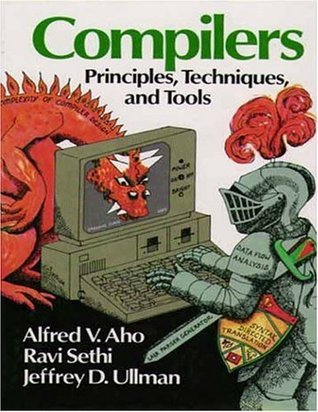
\includegraphics[width=\textwidth]{img/presentation/intro-dragon-book.jpg}
  \end{minipage}
  \hspace{5pt}
  \begin{minipage}[t]{0.2022\textwidth}
    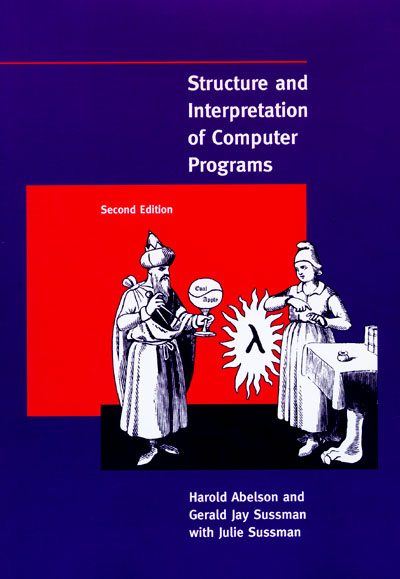
\includegraphics[width=\textwidth]{img/presentation/intro-sicp-book.jpg}
  \end{minipage}
  \label{fig:magic-books}
  \caption{Two classic books in compiler literature.}
\end{figure}
\end{frame}

\begin{frame}[label={sec:orgfc77742}]{Compilers are Indeed Complicated}
A modern compiler toolchain might be composed of:
\begin{itemize}
\item a compiler \emph{frontend:}
\begin{itemize}
\item lexical, syntactic and semantic analysis
\item IR code generation
\end{itemize}
\item a compiler \emph{backend:}
\begin{itemize}
\item optimization passes on the IR
\item target code generation
\item optimization passes on the target code
\end{itemize}
\item an assembler
\item a linker
\end{itemize}

\pause

\dots{} with each stage having seen decades of research \& development!
\end{frame}

\begin{frame}[label={sec:org7e7321c}]{Accessible Compilers}
\begin{quote}
Real-life compilers are too complex to serve as an educational
tool. --- Abdulaziz Ghuloum
\end{quote}

\pause

\begin{itemize}
\item We need easy to understand, educational compilers. \pause
\item Many exist, with various goals and approaches. Distinctions include:
\begin{itemize}
\item Source language: high-level or low-level, existing or devised etc.
\item Target language: bytecode, assembly etc.
\item Implementation language: usually a high-level language (\(\ge\) C).
\item Focus: parsing, code generation, optimizations etc. \pause
\end{itemize}
\item What should our approach be?
\end{itemize}
\end{frame}

\begin{frame}[label={sec:orgb4b0113}]{Goal and Approach}
\begin{itemize}
\item Goal: Show the whole process of implementing a programming language
(within reason). \pause
\item Approach:
\begin{itemize}
\item Source language: \pause Forth. \pause
\item Target language: \pause machine code. \pause
\item Implementation language: \pause machine code! \pause
\item Focus: interfacing with the OS, minimal parsing, code generation,
compiler bootstrapping, extension of the system in the source
language itself etc.
\end{itemize}
\end{itemize}
\end{frame}

\begin{frame}[label={sec:org8b919bf},fragile]{What is Forth?}
 \begin{itemize}
\item Concatenative, ``stack-oriented'' programming language.
\begin{itemize}
\item Data is passed implicitly via the data stack.
\item Reverse Polish notation.
\item Minimalist syntax. \pause
\end{itemize}
\item Another language's \texttt{println(25 * 10 + 50)} becomes:
\begin{verbatim}
25 10 * 50 + . CR
\end{verbatim}
\pause
\item \emph{Word} extension via colon-definitions:
\begin{verbatim}
: SQUARE ( n -- n' )   DUP * ;
\end{verbatim}
\pause
\item Suprising expressivity through mixing compile-time and run-time
effects; similar to Lisp macros.
\end{itemize}
\end{frame}

\begin{frame}[label={sec:orge636368}]{SmithForth}
\begin{itemize}
\item Many existing Forth implementations\dots{}
\item Our favorite: SmithForth\footnote{David Smith, 2022}. \pause
\begin{itemize}
\item Written in machine-code and Forth (once bootstrapped).
\item Targets the x86-64 architecture.
\item Relies on Linux system calls. \pause
\end{itemize}
\item Idea: port SmithForth to a different architecture! \pause
\begin{itemize}
\item Explore two ``competing'' architectures. \pause
\item Learn some low-level Linux interfaces. \pause
\item Deeply understand how a real language is implemented.
\end{itemize}
\end{itemize}
\end{frame}

\begin{frame}[label={sec:org3ca087c}]{From x86-64 Forth to RISC-V}
\begin{itemize}
\item RISC-V chosen as porting target.
\begin{itemize}
\item Modern, simple, elegant, ``up-and-coming'' ISA.
\item Modular design: ISA = base-ISA + extensions.
\item We only use the 64-bit base ISA with no extensions.
\end{itemize}
\end{itemize}
\end{frame}

\begin{frame}[label={sec:orgcb25b1d}]{The Plan}
\begin{enumerate}
\item Understand and annotate SmithForth's machine code:
\begin{itemize}
\item Create detailed pseudocode showing how it works.
\item Make x86-64 instruction encodings explicit. \pause
\end{itemize}
\item Port SmithForth's machine code to RISC-V.
\begin{itemize}
\item Follow the pseudocode produced in the previous step.
\item Adapt to RISC-V's idiosyncrasies. \pause
\end{itemize}
\item We now have a basic Forth system.
\begin{itemize}
\item Extend it further in Forth itself!
\item Prove that we have a usable system.
\end{itemize}
\end{enumerate}
\end{frame}


\section{SmithForth: Annotation and Analysis}
\label{sec:org0be7aad}

\begin{frame}[label={sec:org220c53e}]{Showcase: Handwritten ELF Header}
\begin{figure}[htbp]
\centering
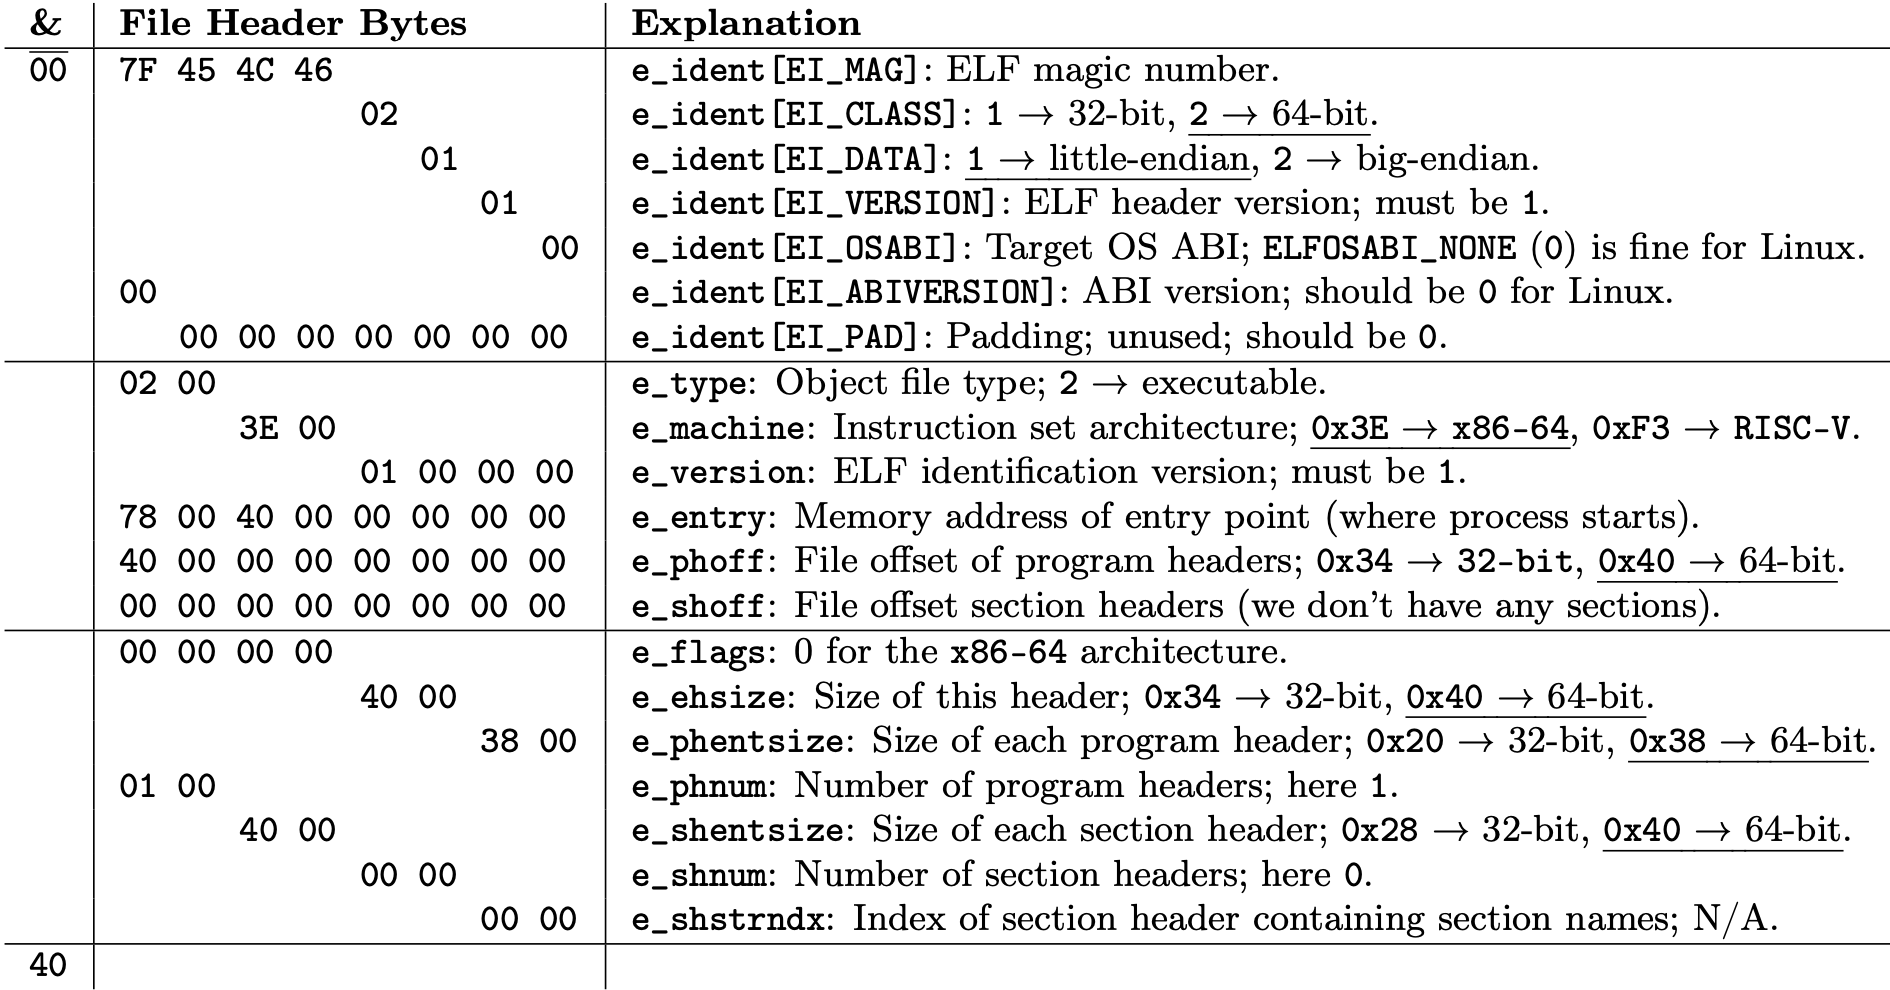
\includegraphics[width=0.98\textwidth]{img/presentation/elf-header.png}
\caption{The beginning of SmithForth's handmade executable.}
\end{figure}
\end{frame}

\begin{frame}[label={sec:orge2d80bd},fragile]{Showcase: Subroutine \texttt{PARSE} -- Before}
 \fontsize{7ptpt}{8.400000pt}\selectfont
\begin{verbatim}
99 05 50 41 52 53 45 ## PARSE ( cl dl "ccc<char>" -- rbp=addr rax=u )
49 C7 C1 00 00 00 10  # r9 = VAR              mov r/m64, imm32   REX.W C7 /0 id   11 000 001
49 8B 69 10           # rbp = [>IN]           mov r64, r/m64     REX.W 8B /r      01 101 001
99 73                 # Call seek				        		      
49 8B 41 10           # rax = [>IN]           mov r64, r/m64     REX.W 8B /r      01 000 001
73 04                 #+jump _end if U>=   00 jae rel8           73 cb	      
49 FF 41 10           # [>IN]++               inc r/m64          REX.W FF /0      01 000 001
# _end:               #                    04		        		      
48 29 E8              # rax -= rbp            sub r/m64, r64     REX.W 29 /r      11 101 000
49 03 69 08           # rbp += [TIB]          add r64, r/m64     REX.W 03 /r      01 101 001
C3                    # return                ret                C3    
\end{verbatim}
\captionof{figure}{Machine code definition of \texttt{PARSE} (original SmithForth).}
\normalsize
\end{frame}

\begin{frame}[label={sec:org3ae3e4b},fragile]{Showcase: Subroutine \texttt{PARSE} -- After}
 \begin{figure}[htbp]
\centering
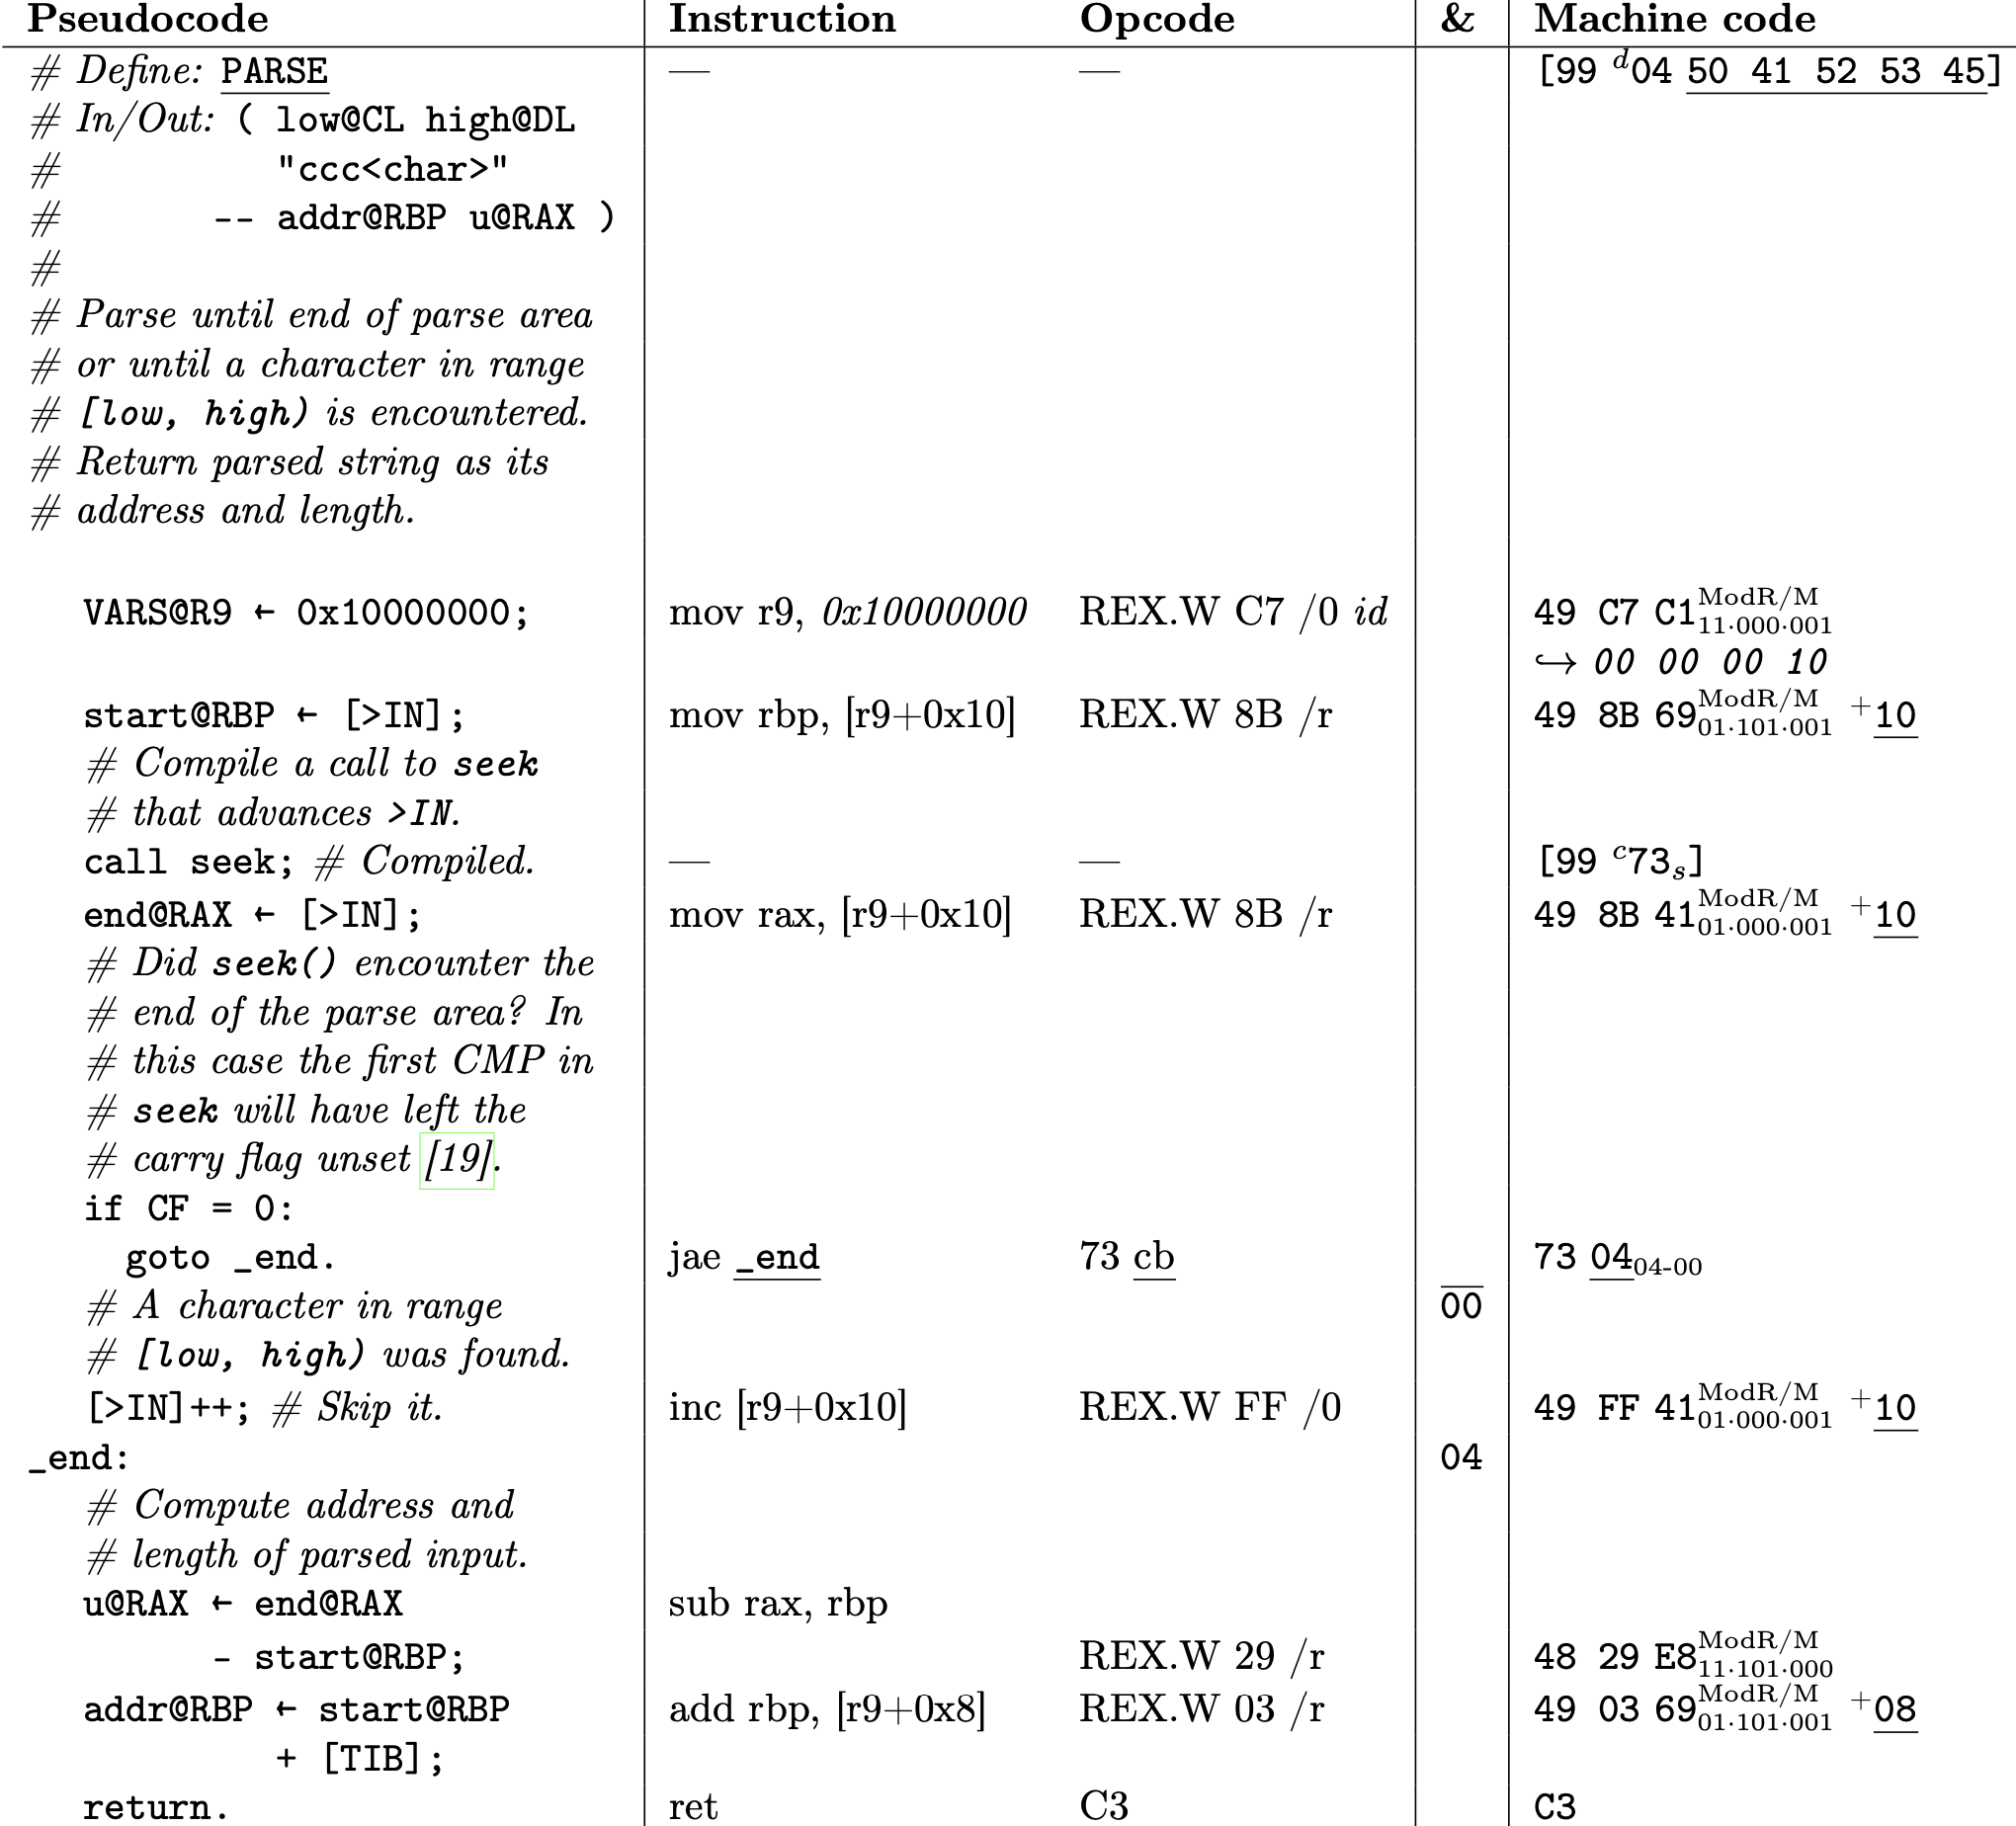
\includegraphics[width=0.70\textwidth]{img/presentation/PARSE-annotated.png}
\caption{Machine code definition of \texttt{PARSE} (annotated SmithForth).}
\end{figure}
\end{frame}

\section{Porting SmithForth to RISC-V}
\label{sec:orgee58550}

\begin{frame}[label={sec:org3ff56d8},fragile]{Showcase: Subroutine \texttt{PARSE} -- RISC-V}
 \begin{figure}[htbp]
\centering
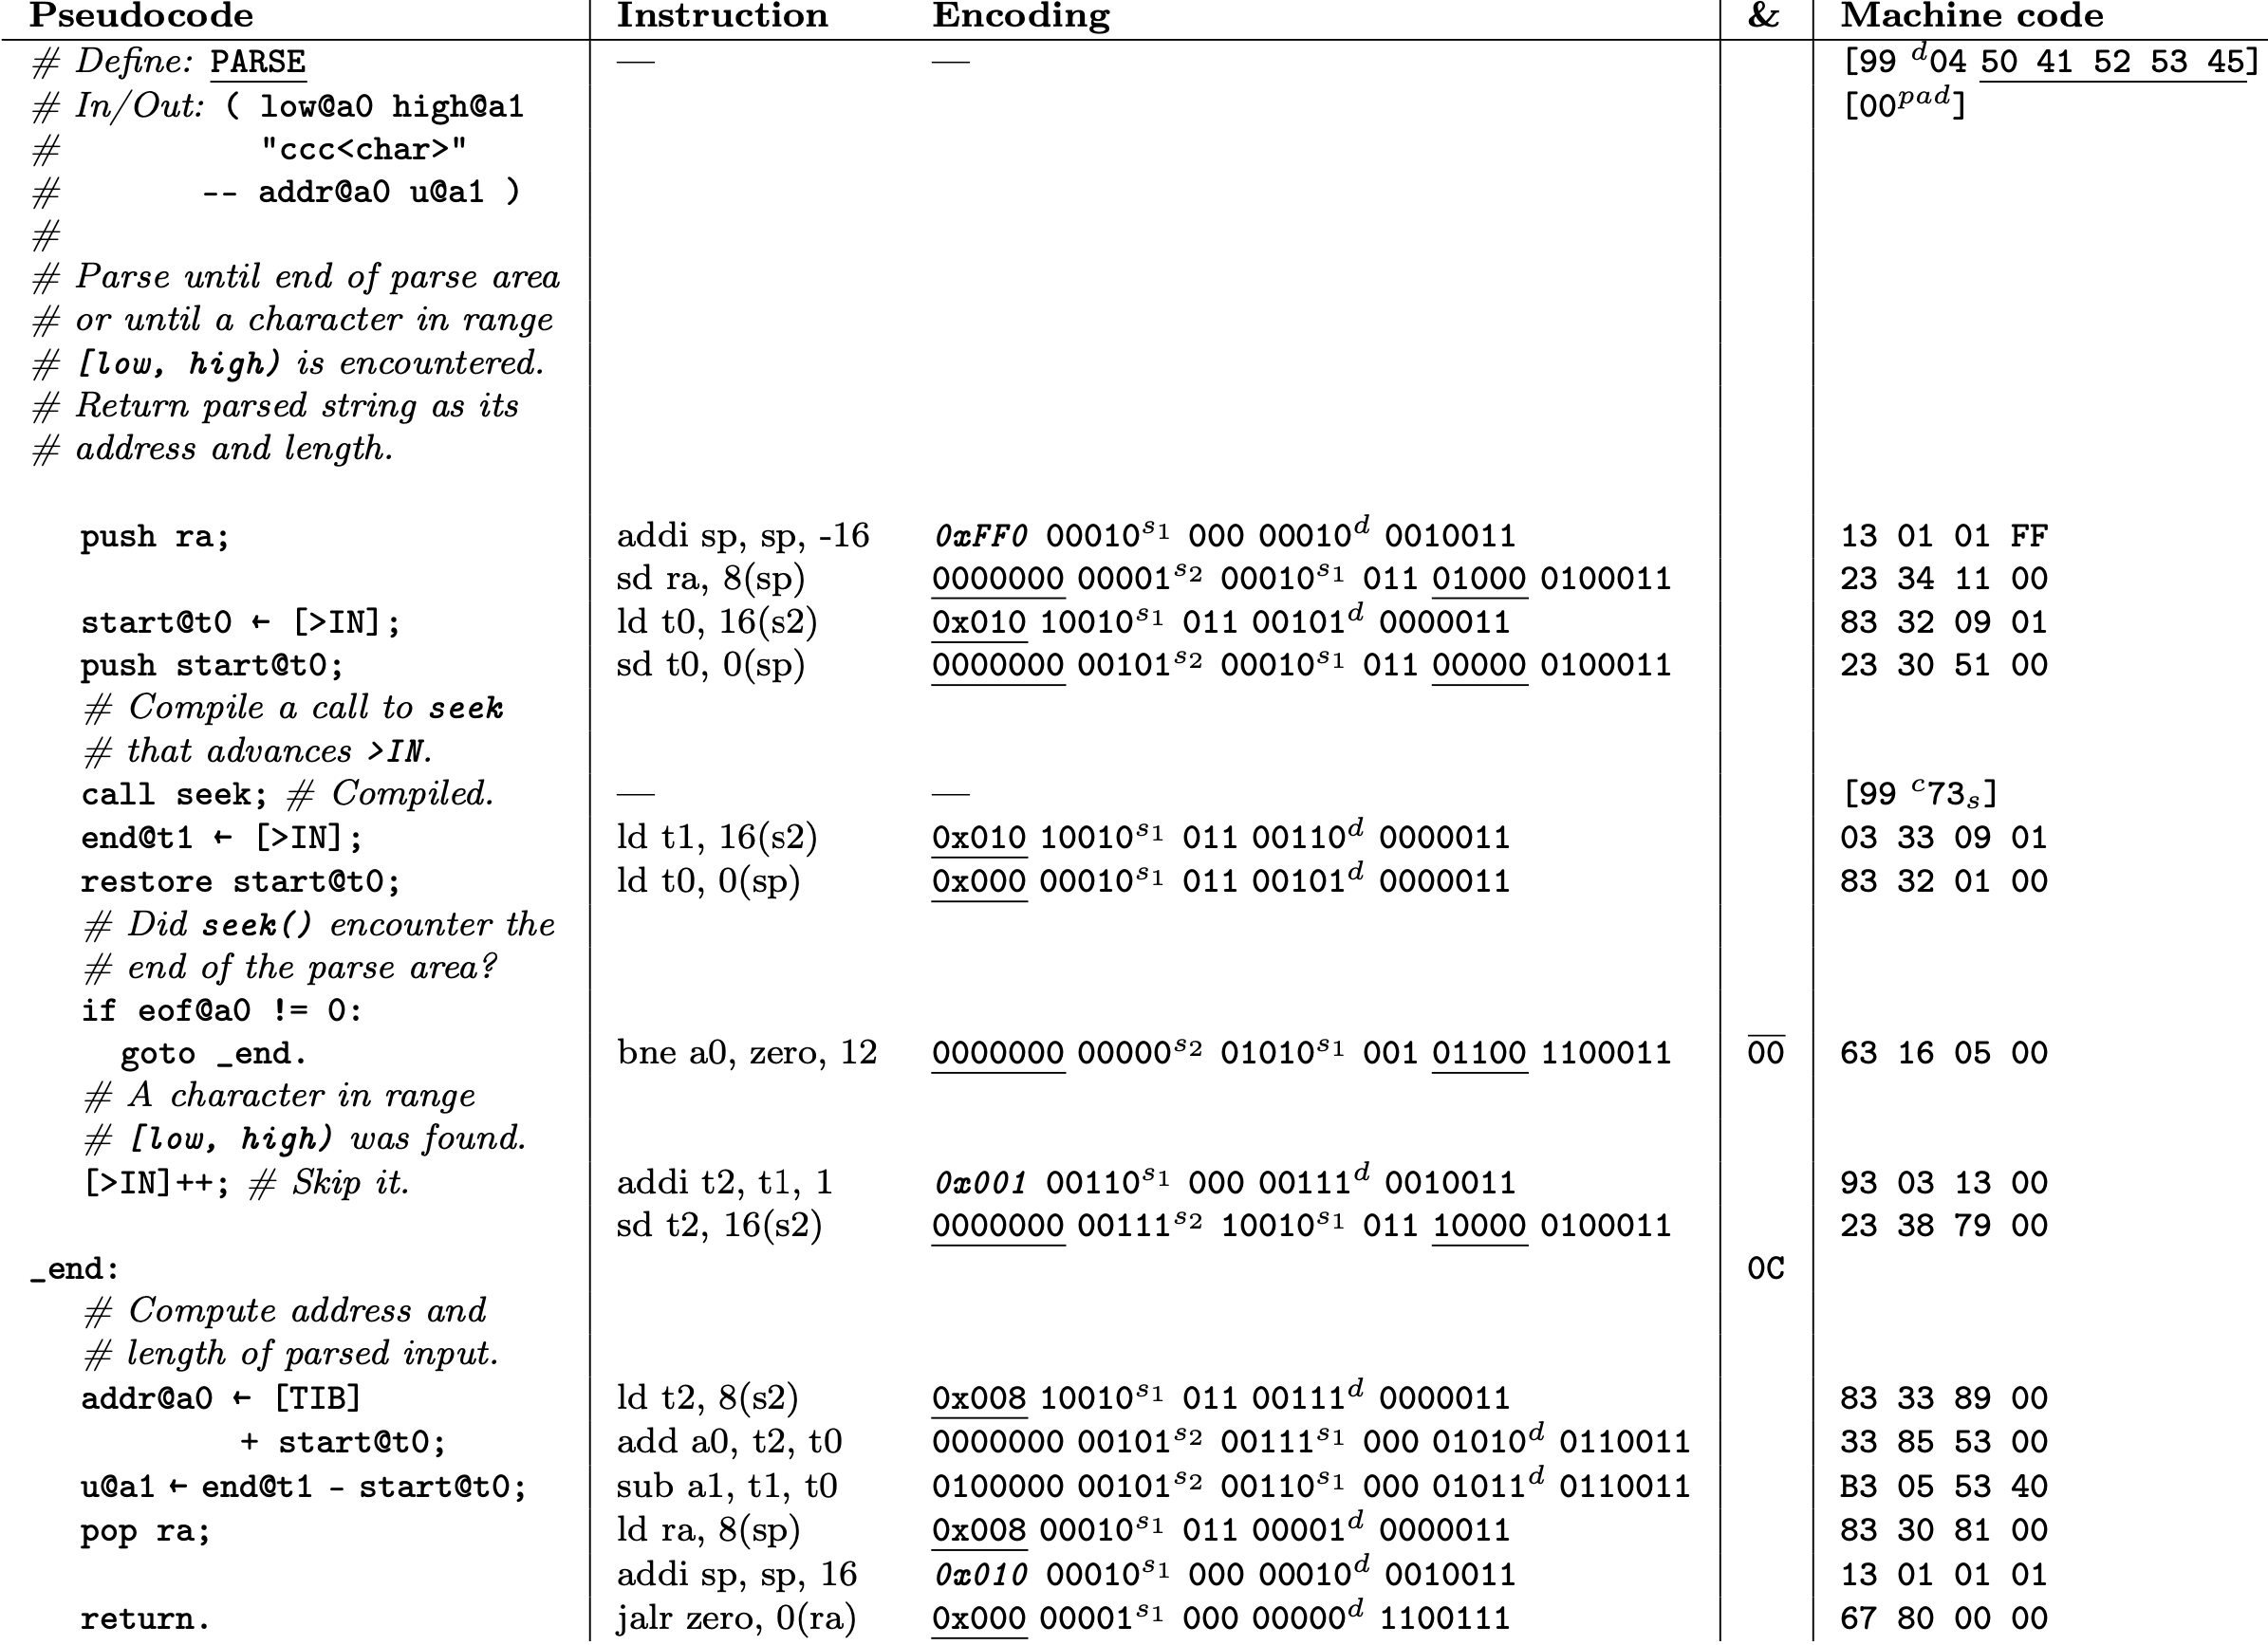
\includegraphics[width=0.87\textwidth]{img/presentation/PARSE-riscv.png}
\caption{Machine code definition of \texttt{PARSE} (RISC-V port).}
\end{figure}
\end{frame}


\section{Forth in Forth}
\label{sec:org5a8e7ae}

\begin{frame}[label={sec:orgd230fdc}]{Showcase: A RISC-V Assembler in Forth}
\begin{figure}[htbp]
\centering
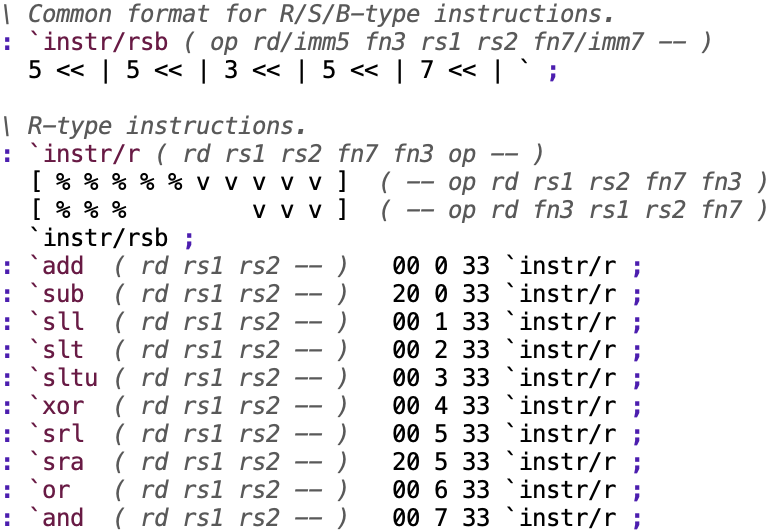
\includegraphics[width=0.61\textwidth]{img/presentation/forth-assembler.png}
\caption{Defining RV32I R-type instructions in Forth.}
\end{figure}
\end{frame}

\begin{frame}[label={sec:orgae2f9ef}]{Showcase: Forth's Arithmetic Operators}
\begin{figure}[htbp]
\centering
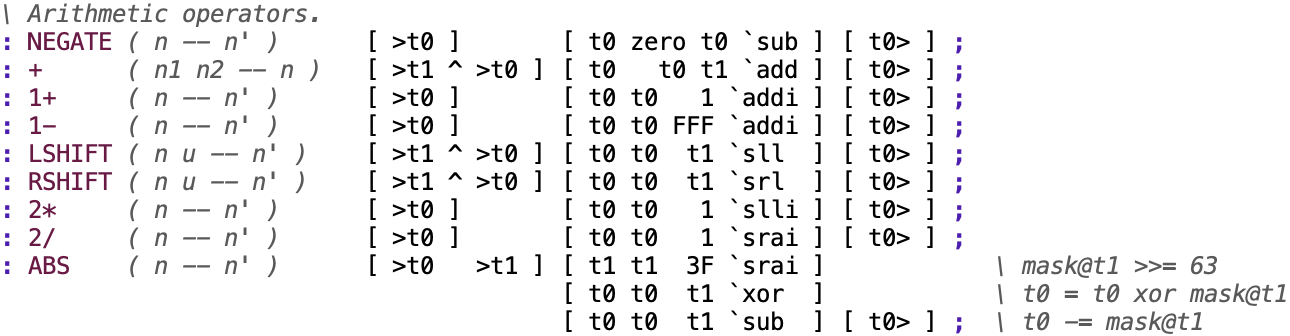
\includegraphics[width=0.95\textwidth]{img/presentation/forth-arithmetic.png}
\caption{Defining Forth's basic arithmetic operators using the assembler.}
\end{figure}
\end{frame}

\begin{frame}[label={sec:org8a4d2e5}]{Showcase: Usable enough for FizzBuzz}
\begin{figure}[htbp]
\centering
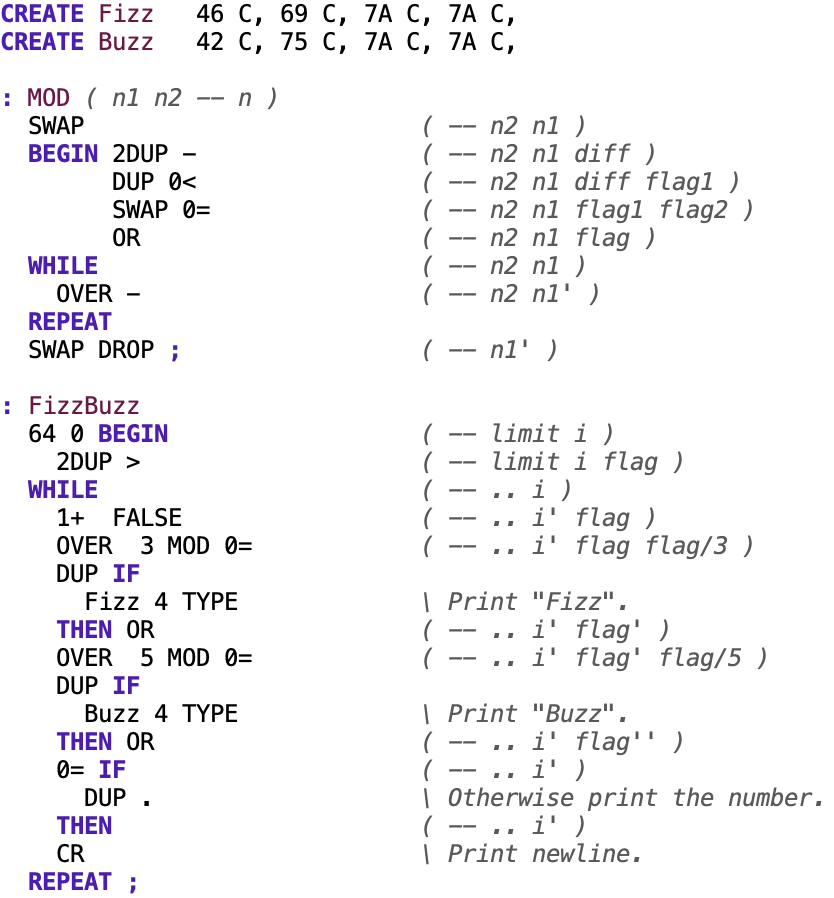
\includegraphics[width=0.60\textwidth]{img/presentation/forth-fizz-buzz.png}
\caption{Solving FizzBuzz in Forth.}
\end{figure}
\end{frame}


\section{Conclusions}
\label{sec:org489dbe3}

\begin{frame}[label={sec:orge80e3fe}]{Summary \& Conclusions}
\begin{itemize}
\item We implemented a basic Forth system ``from scratch'', using only
handwritten RISC-V machine code and several Linux system calls.  We
used the excellent SmithForth x86-64 implementation as reference and
inspiration. \pause
\item We extended the Forth system in Forth itself, implementing basic
primitives, a RISC-V assembler, common arithmetic, logic \&
comparison operators, control flow constructs and, finally, a
solution to the FizzBuzz problem to prove the usability of our
system. \pause
\item Both process and code were clearly explained and annotated.  Our
accessible Forth implementation illustrates how abstraction builds
upon abstraction along the path from elementary processor
instructions to powerful high-level languages.
\end{itemize}
\end{frame}
\end{document}
